\section{Lernziel AO: Performance von Datenbank-Anfragen optimieren}

\subsection{Leistungsengpässe verstehen: Join, quadratische Komplexität}

Eine Datenbankabfrage wird langsamer wenn mehr Ergebnisse (grössere Tabellen) verarbeitet werden müssen. Bei einem Join werden zwei oder mehr Tabellen miteinander verknüpft und so mehr Ergebnisse produziert. Durch einen Join wird eine Abfrage folglich langsamer. Ein sogenannter \emph{nested join} hat eine quadratische Komplexität. Bei einem \emph{nested join} werden alle Tupel aus der Tabelle A nacheinander mit den Tupeln aus der Tabelle B verglichen. Eine schneller Abfrage könnte man erreichen wenn man eine Spalte mit Index vergleicht. 

\subsection{SQL-Anfragen logisch optimieren via Anfragebaum}

SQL-Anfragen können als Anfragebaum grafisch dargestellt werden (siehe Lernziel \ref{sec:anfragebaum}). Abbildung \ref{fig:anfrageoptimierung} zeigt eine Anfrageoptimierung auf welche folgende Regeln angewendet wurden:

\begin{enumerate}
	\item Mehrere Selektionen auf die gleiche Tabelle zu einer Selektion zusammenfassen.
	\item Tabellen immer klein halten:
		\begin{enumerate}
			\item Möglichst kleine Zwischenresultate.
			\item Nicht benötigte Zeilen und Spalten aus Tabelle entfernen (Selektion, Projektion).
			\item Beides möglichst früh (weit unten im Baum) anwenden.
		\end{enumerate}
	\item Join im Wurzelknoten des Baumes verwenden (erst am ganz am Schluss).
\end{enumerate}

\begin{figure}[h!]
	\centering
	\begin{subfigure}[b]{0.3\textwidth}
		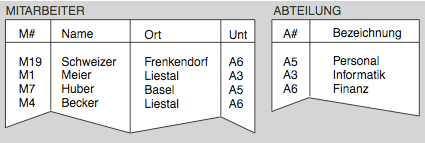
\includegraphics[width=\textwidth]{fig/anfrage_tabellen.png}
		\caption{Tabellen der Anfrage}
	\end{subfigure}
	\begin{subfigure}[b]{0.3\textwidth}
		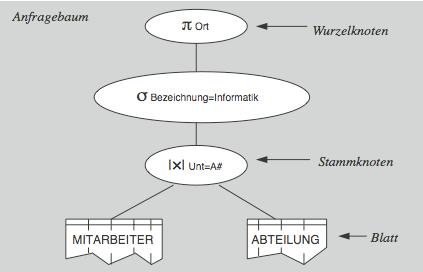
\includegraphics[width=\textwidth]{fig/anfrage_nicht_optimiert.png}
		\caption{Anfrage nicht optimiert}
	\end{subfigure}
	\begin{subfigure}[b]{0.3\textwidth}
		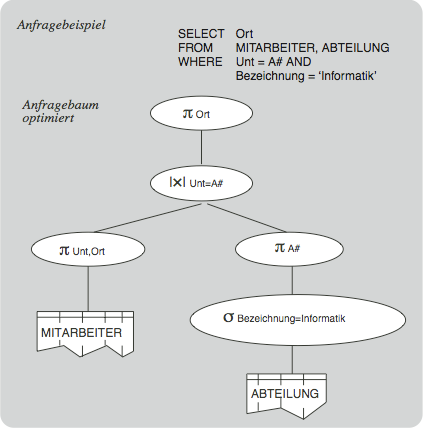
\includegraphics[width=\textwidth]{fig/anfrage_optimiert.png}
		\caption{Anfrage optimiert}
	\end{subfigure}
	\caption{Anfrageoptimierung}
	\label{fig:anfrageoptimierung}
\end{figure} 

\subsection{Indexe sinnvoll setzen und verwenden (Primary Key, Foreign Key, Attribute)}

Ein Index ist eine Baumstruktur mit welcher Datensätze schnell aufgefunden werden können (Inhaltsverzeichnis von Buch). Für Primary und Foreign Keys werden Indexe automatisch angelegt. Für sonstige Attribute muss ein Index manuell gesetzt werden (Listing \ref{lst:index}). Ein Index sollte auf Attributen gesetzt werden die oft durchsucht werden (Index sparsam einsetzen).

\begin{lstlisting}[caption={Index erstellen},label=lst:index]
CREATE INDEX index_name ON table_name (column_name)
\end{lstlisting}

\subsection{Einen Execution-Plan im Datenbankserver anzeigen und auswerten}

Listing \ref{lst:explain} zeigt wie ein Execution-Plan erstellt wird.

\begin{lstlisting}[caption={Execution-Plan anzeigen},label=lst:explain]
EXPLAIN select * from Professoren
\end{lstlisting}